\section{Results}

\subsection{Residual Map}
\begin{itemize}
    \item Show one of each of the type of models used to make the residual map. Possibly include the entire image in appendix or link to a fits file containing the image.
    \item Stats from the modelling. How many of each type, which is the most common etc. How many models failed.
    \item Mention the masks (maybe in method instead) covering bright spots that are not included in the cosmos catalogue since they were corrupt.
    \item Think about running the source detection on this image as was the plan and provide some stats of the result.
    \item Mention that we ended up using the residual image Iary made weighing the channel 1 and 2 images of IRAC. Explain quickly how this was made, and why we believe it to be more robust than the residual map I myself created. Elaborate on this in the discussion. The FARMER catalogue is still not finished developed
\end{itemize} 

\begin{wrapfigure}{r}{0.4\textwidth}
    \centering %left, lower, right, upper
    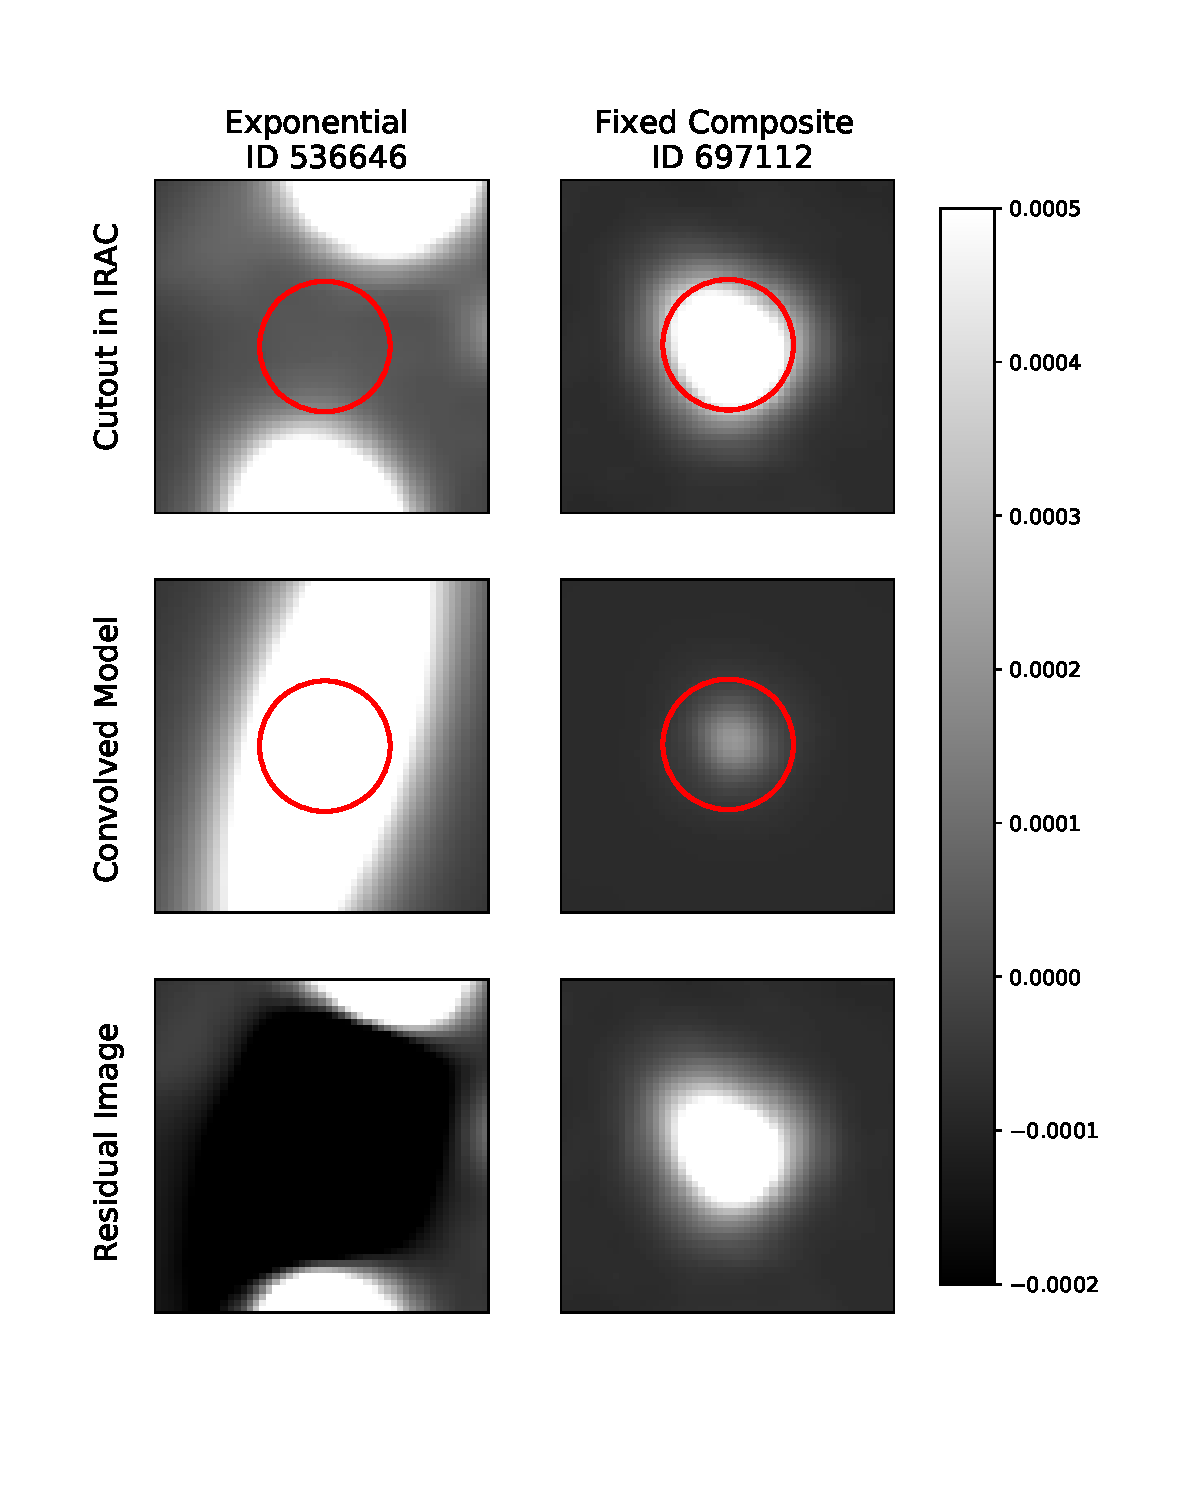
\includegraphics[trim={1cm 2.5cm 2cm 1.5cm},clip,width=0.38\textwidth]{Code/Saved_Figures/BAD_model_cutouts.pdf}
    \caption{hi}
    \label{BAD_Model_cutouts}  
\end{wrapfigure}

\begin{figure}[h!]
    \centering
    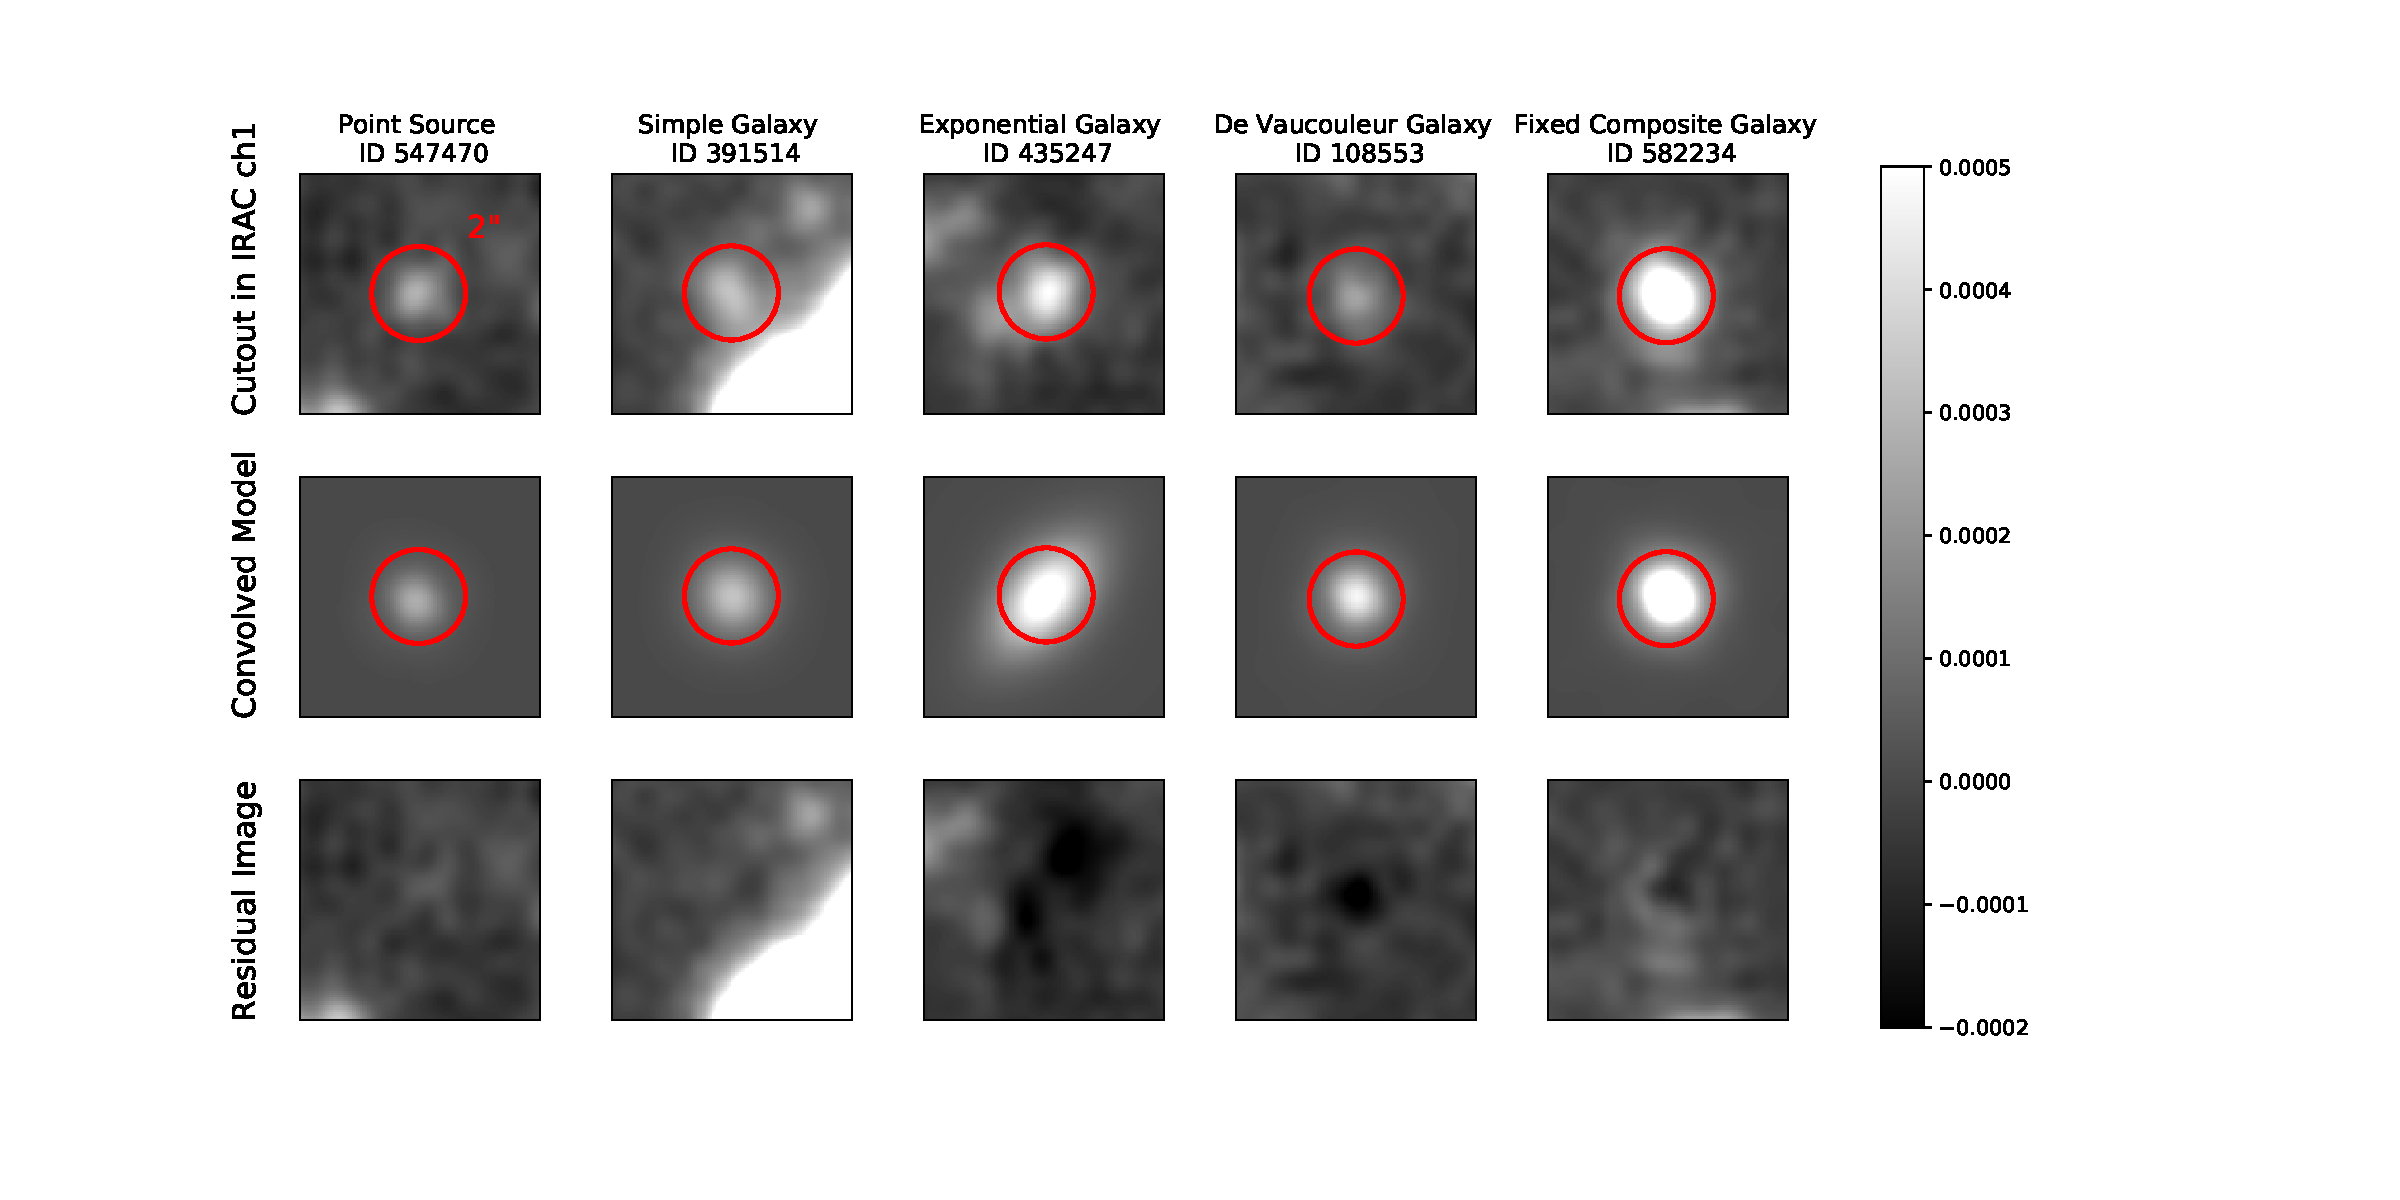
\includegraphics[trim={3cm 2.5cm 5cm 1.5cm},clip,scale=0.5]{Code/Saved_Figures/Model_cutouts.pdf}
    \caption{hi}
    \label{Model_cutouts}
\end{figure}

\subsection{Dimensionality Reduction}
\begin{itemize}
    \item t-SNE embedding plot with varying perplexities and colors (blue-red) colormapped. Describe the corrupted flux marked in another color. Include the most interesting one - "k-c1" here, "h-k" and "ch1-ch2" can be added in the appendix.
    \item Describe why that perplexity is chosen. Describe the color distribution. There are two outliers or so that fall distant from the main cluster, quickly look to these and describe why we omit them from the analysis.
    \item Describe our use of tracers - how many good ones were there and a few stats.
    \item Show the results on the chosen perplexity. Main plot = t-SNE embedding where the matched objects, good candidates and fluxes above some threshold is colormapped. This allows us to mark three regions, and we display cutouts from at least one object in each region as subplots around the embedding plot.
\end{itemize}

\begin{figure}[h!]
    \centering %left, lower, right, upper
    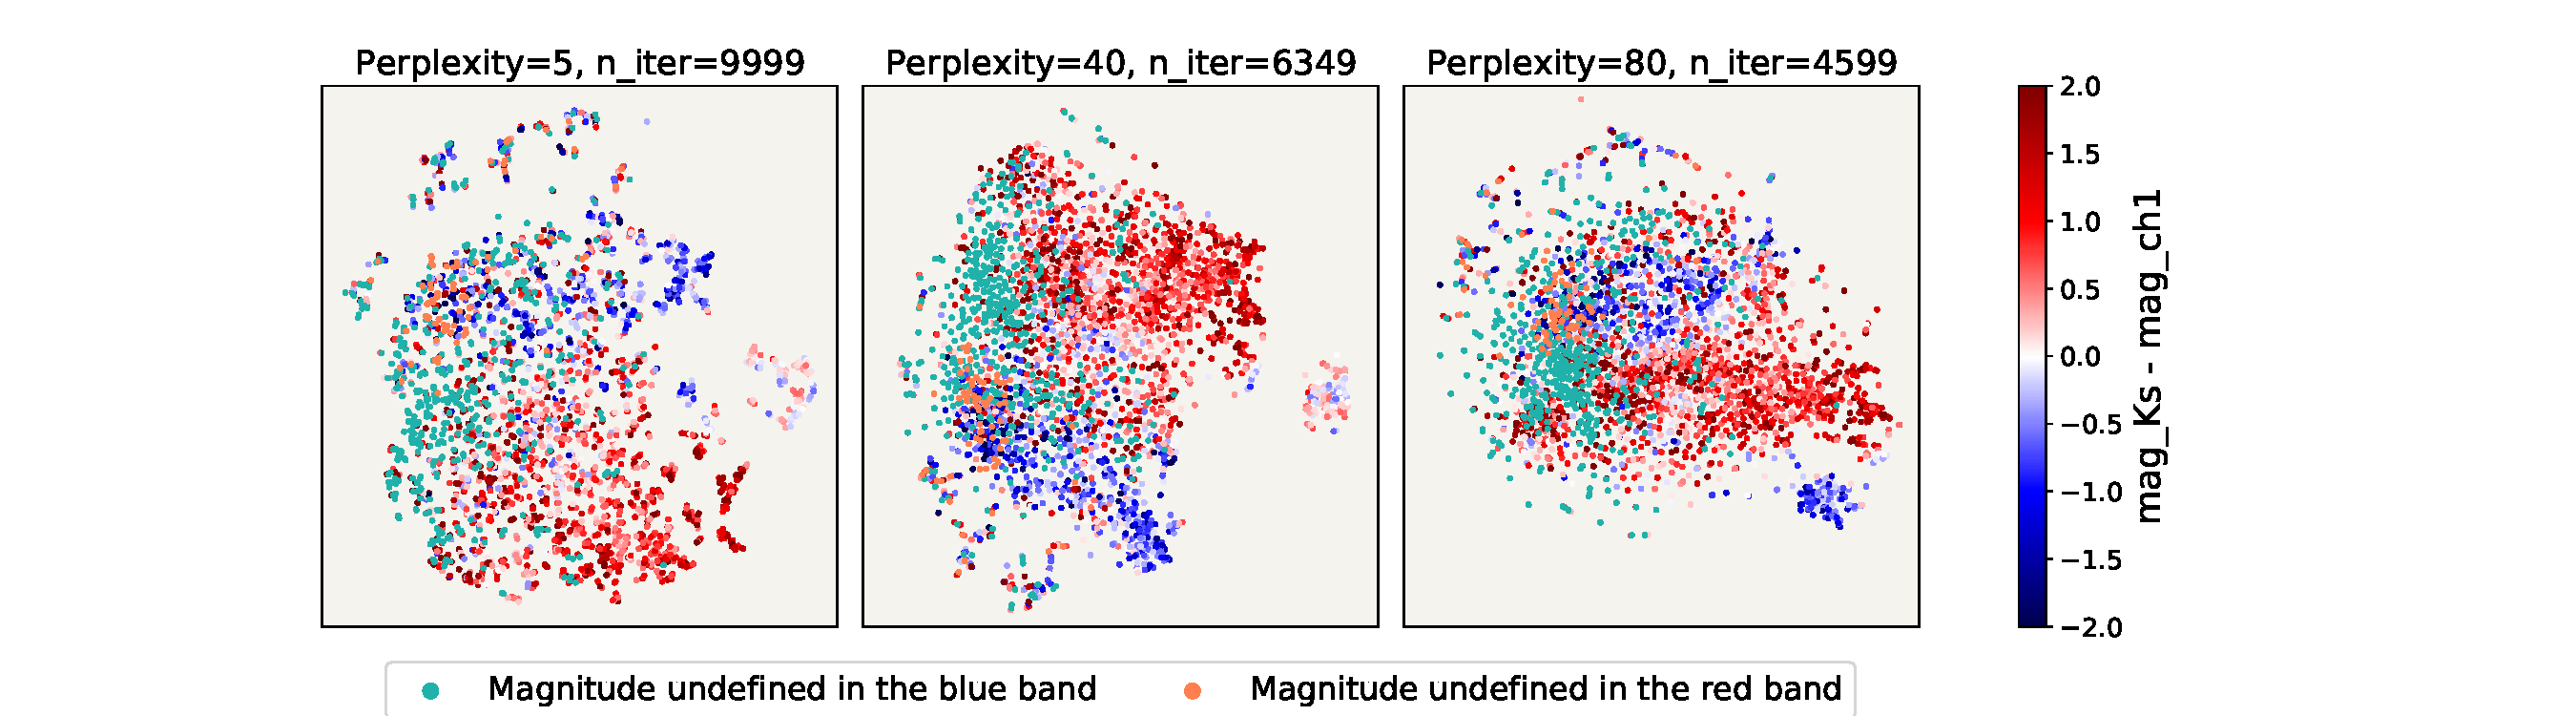
\includegraphics[trim={5cm 0cm 5cm 0.5cm},clip,width=\textwidth]{Code/Saved_Figures/peplex_Ks_ch1_SMALL.pdf}
    \caption{hi}
    \label{SMALL_embeddding_ks_ch1}
\end{figure}

Perplexity 40 is chosen since the result is a nice cluster with clearly seperated blue and red galaxies (see figure \ref{SMALL_embeddding_ks_ch1}). Additionally the n-iter ended up 6349 whcih is less than max-iter of 10000, meaning that the embedding converged. Peplexity 80 and 100 also converged but the original paper \cite{Maaten_2008_tSNE} suggests choosing perplexities between 5 and 50. All perplexities tested is seen in appendix along with the color between the other bands.

\subsection{Classification / Identifying Promising Candidates}
\begin{itemize}
    \item Show the classifications on the embedding. Two subplots, one showing the embedding colores according to the labels that are known to the algorithm and one according to the predicted labels.
    \item Acompany this with a score metric. Accuracy, contamination rate and a confusion matrix are good scores to show. And write which parameters where chosen, what is k, what is fmin and so on.
    \item Produce the plot we talked about in mondays meeting similar to figure 4 in \cite{Steinhardt_2020}. A plot as a function of fmin showing contamination and the size of each population (good and bad) acompanied with a ROC curve.
    \item Include the SED plots, and show that our candidates look as we expect. Faint in H and K and more bright in ch1 and ch2.
\end{itemize}

\begin{figure}[h!]
    \centering %left, lower, right, upper
    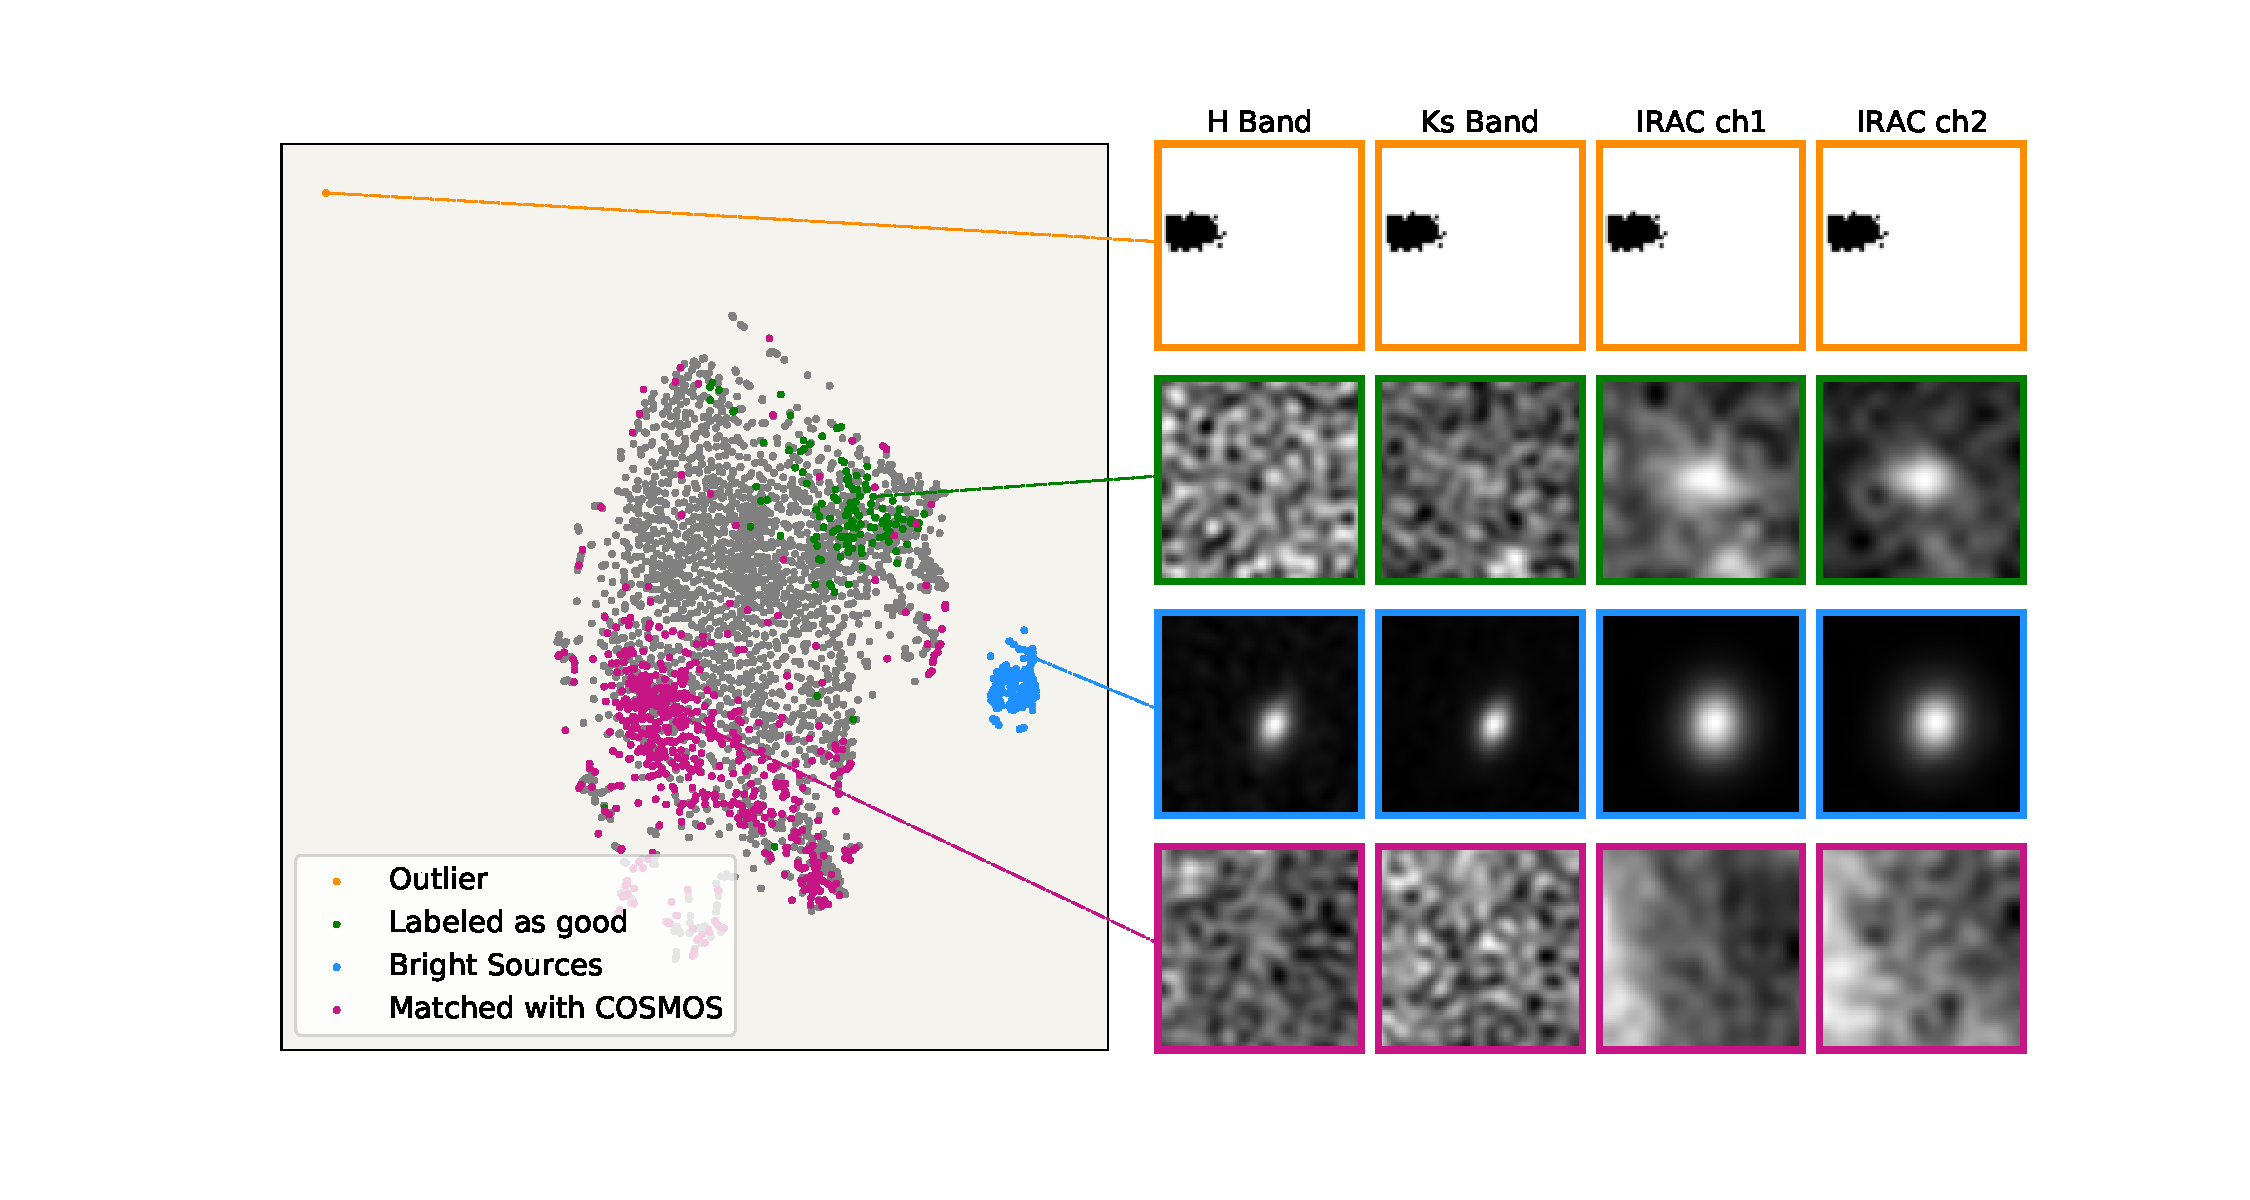
\includegraphics[trim={0cm 0cm 0cm 0cm},clip,width=\textwidth]{Code/Saved_Figures/Visual_inspection_embedding.pdf}
    \caption{hi}
    \label{embedding_regions}
\end{figure}

\begin{figure}[h!]
    \centering %left, lower, right, upper
    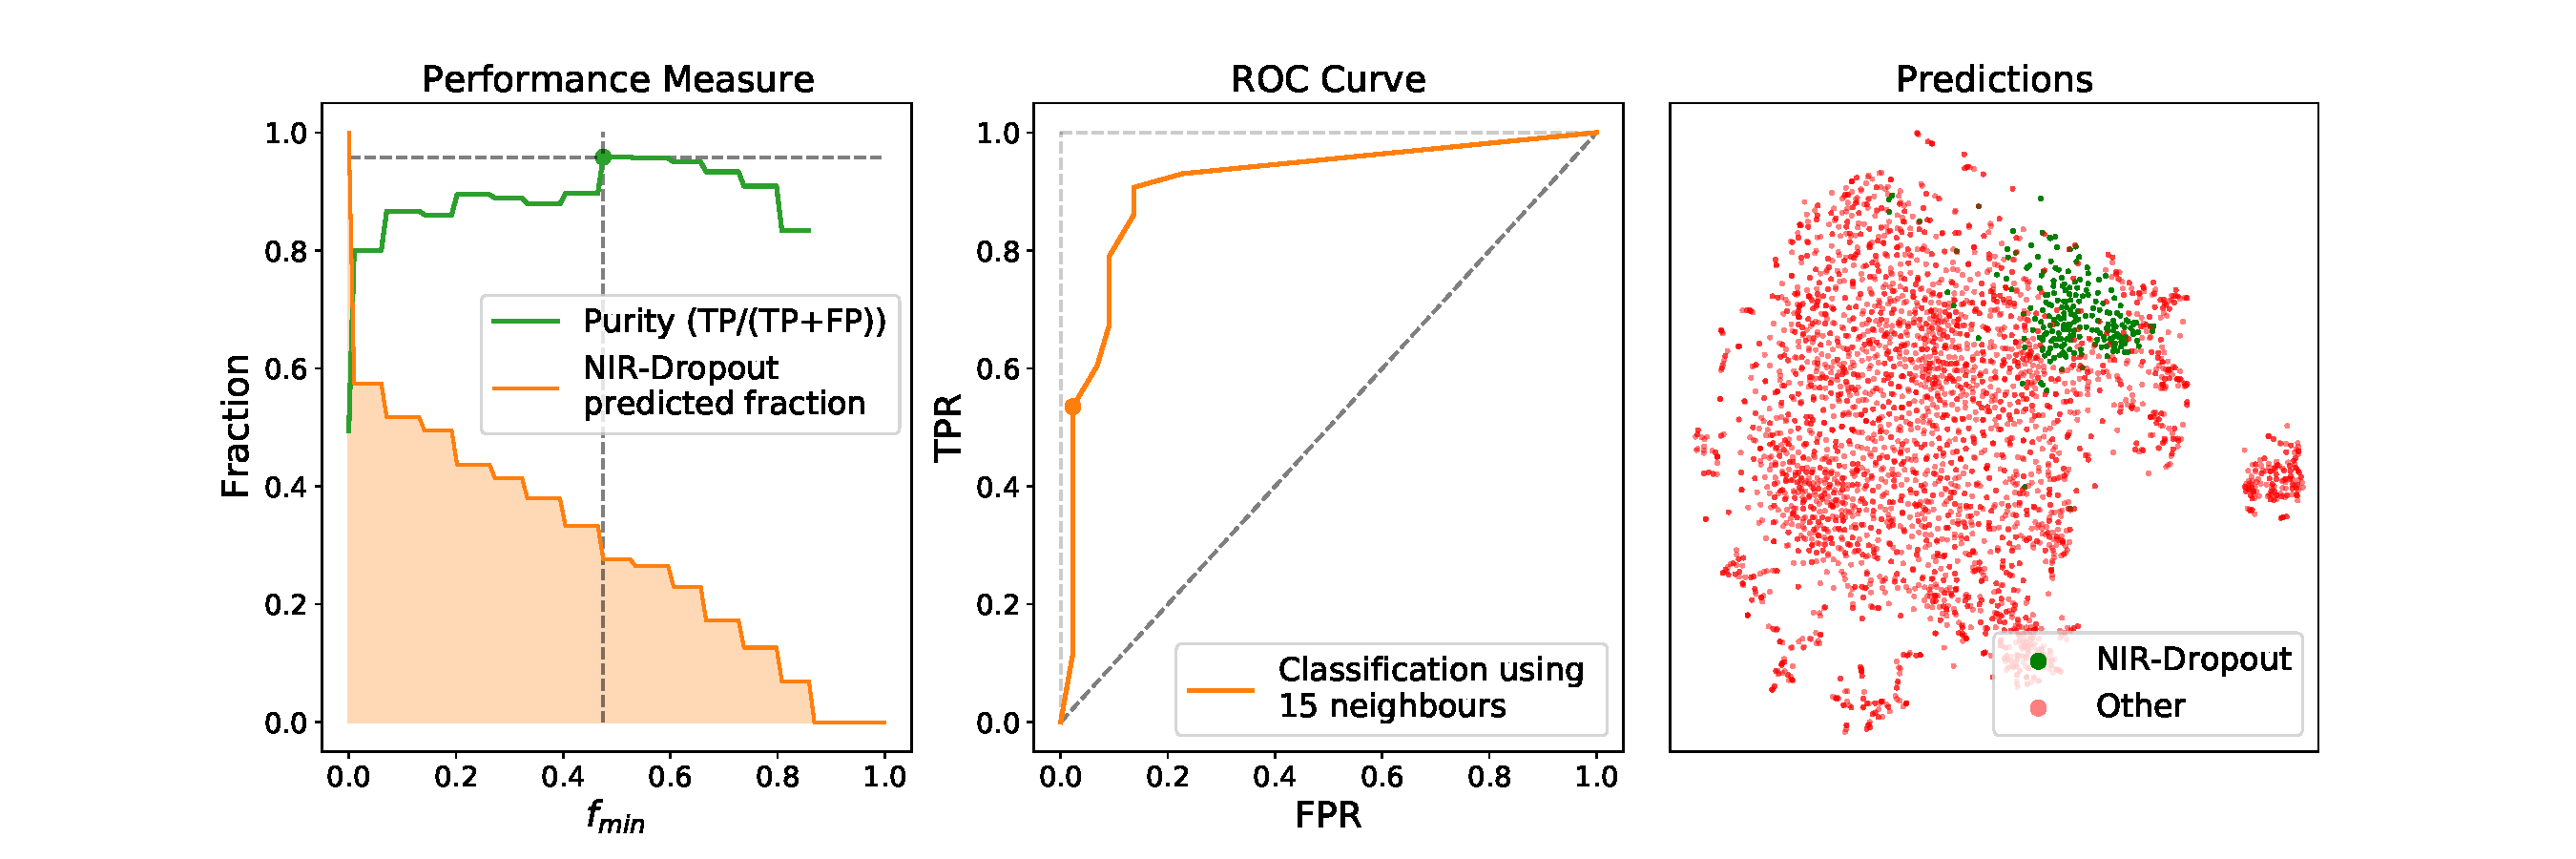
\includegraphics[trim={3.5cm 0cm 4.5cm 0cm},clip,width=\textwidth]{Code/Saved_Figures/Classification_plot.pdf}
    \caption{hi}
    \label{classification_plot}
\end{figure}